\documentclass{standalone}
\usepackage{tikz}
\usetikzlibrary{patterns, positioning}


\begin{document}
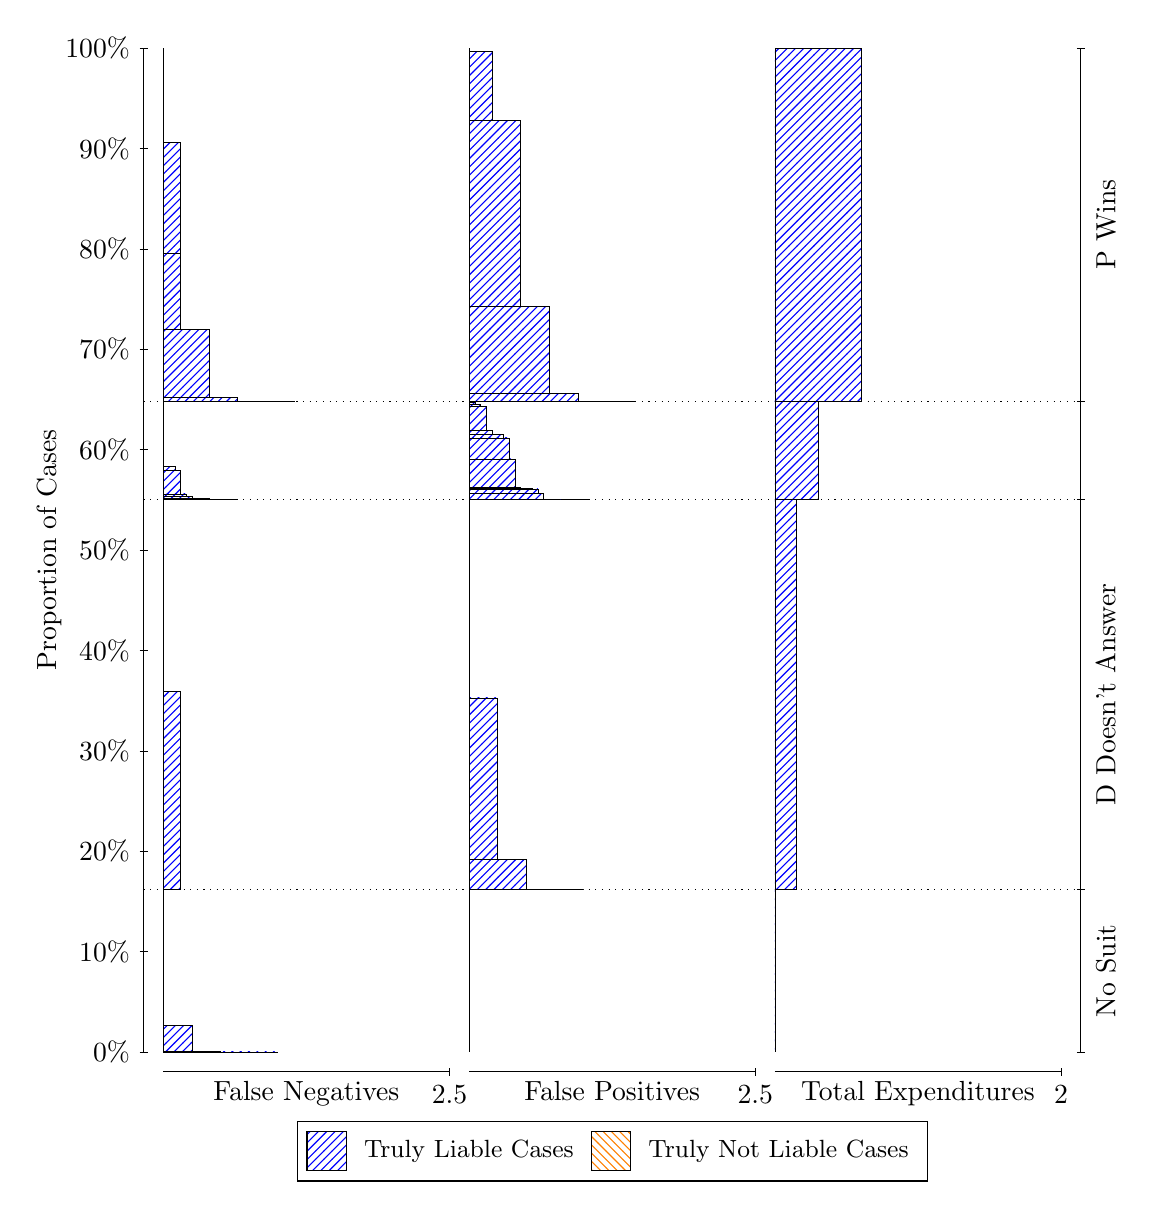
\begin{tikzpicture}
\draw[black, very thin] (1.5,1.75) -- (1.5,14.5);
\node[rotate=90, text=black, anchor=center] at (0.3, 8.125) {Proportion of Cases};
\draw[black, very thin] (1.45,1.75) -- (1.55,1.75);
\node[text=black, anchor=east] at (1.45, 1.75) {0\%};
\draw[black, very thin] (1.45,3.025) -- (1.55,3.025);
\node[text=black, anchor=east] at (1.45, 3.025) {10\%};
\draw[black, very thin] (1.45,4.3) -- (1.55,4.3);
\node[text=black, anchor=east] at (1.45, 4.3) {20\%};
\draw[black, very thin] (1.45,5.575) -- (1.55,5.575);
\node[text=black, anchor=east] at (1.45, 5.575) {30\%};
\draw[black, very thin] (1.45,6.85) -- (1.55,6.85);
\node[text=black, anchor=east] at (1.45, 6.85) {40\%};
\draw[black, very thin] (1.45,8.125) -- (1.55,8.125);
\node[text=black, anchor=east] at (1.45, 8.125) {50\%};
\draw[black, very thin] (1.45,9.4) -- (1.55,9.4);
\node[text=black, anchor=east] at (1.45, 9.4) {60\%};
\draw[black, very thin] (1.45,10.675) -- (1.55,10.675);
\node[text=black, anchor=east] at (1.45, 10.675) {70\%};
\draw[black, very thin] (1.45,11.95) -- (1.55,11.95);
\node[text=black, anchor=east] at (1.45, 11.95) {80\%};
\draw[black, very thin] (1.45,13.225) -- (1.55,13.225);
\node[text=black, anchor=east] at (1.45, 13.225) {90\%};
\draw[black, very thin] (1.45,14.5) -- (1.55,14.5);
\node[text=black, anchor=east] at (1.45, 14.5) {100\%};

\draw[black, very thin] (13.4,1.75) -- (13.4,14.5);
\draw[black, very thin] (13.35,1.75) -- (13.45,1.75);
\node[anchor=west] at (13.35, 1.75) {};
\draw[black, very thin] (13.35,3.8119) -- (13.45,3.8119);
\node[anchor=west] at (13.35, 3.8119) {};
\draw[black, very thin] (13.35,8.7655) -- (13.45,8.7655);
\node[anchor=west] at (13.35, 8.7655) {};
\draw[black, very thin] (13.35,10.016) -- (13.45,10.016);
\node[anchor=west] at (13.35, 10.016) {};
\draw[black, very thin] (13.35,14.5) -- (13.45,14.5);
\node[anchor=west] at (13.35, 14.5) {};

\draw[black, very thin, pattern color=blue, pattern=north east lines] (1.75,1.75) rectangle (3.2033,1.75);
\draw[black, very thin, pattern color=blue, pattern=north east lines] (1.75,1.75) rectangle (2.84,1.75);
\draw[black, very thin, pattern color=blue, pattern=north east lines] (1.75,1.75) rectangle (2.4767,1.7529);
\draw[black, very thin, pattern color=blue, pattern=north east lines] (1.75,1.7529) rectangle (2.1133,2.0876);
\draw[black, very thin, pattern color=orange, pattern=north west lines] (1.75,2.0876) rectangle (1.75,2.0876);
\draw[black, very thin, pattern color=blue, pattern=north east lines] (1.75,2.0876) rectangle (1.75,3.8119);
\draw[black, very thin, pattern color=blue, pattern=north east lines] (1.75,3.8119) rectangle (1.968,6.3315);
\draw[black, very thin, pattern color=orange, pattern=north west lines] (1.75,6.3315) rectangle (1.75,6.3315);
\draw[black, very thin, pattern color=blue, pattern=north east lines] (1.75,6.3315) rectangle (1.75,8.7655);
\draw[black, very thin, pattern color=blue, pattern=north east lines] (1.75,8.7655) rectangle (2.6947,8.7655);
\draw[black, very thin, pattern color=blue, pattern=north east lines] (1.75,8.7655) rectangle (2.404,8.7655);
\draw[black, very thin, pattern color=blue, pattern=north east lines] (1.75,8.7655) rectangle (2.3313,8.7763);
\draw[black, very thin, pattern color=blue, pattern=north east lines] (1.75,8.7763) rectangle (2.2587,8.7788);
\draw[black, very thin, pattern color=blue, pattern=north east lines] (1.75,8.7788) rectangle (2.1133,8.8025);
\draw[black, very thin, pattern color=blue, pattern=north east lines] (1.75,8.8025) rectangle (2.0407,8.8367);
\draw[black, very thin, pattern color=blue, pattern=north east lines] (1.75,8.8367) rectangle (1.968,9.1371);
\draw[black, very thin, pattern color=blue, pattern=north east lines] (1.75,9.1371) rectangle (1.8953,9.1862);
\draw[black, very thin, pattern color=orange, pattern=north west lines] (1.75,9.1862) rectangle (1.75,9.1862);
\draw[black, very thin, pattern color=blue, pattern=north east lines] (1.75,9.1862) rectangle (1.75,10.016);
\draw[black, very thin, pattern color=blue, pattern=north east lines] (1.75,10.016) rectangle (3.4213,10.016);
\draw[black, very thin, pattern color=blue, pattern=north east lines] (1.75,10.016) rectangle (3.058,10.016);
\draw[black, very thin, pattern color=blue, pattern=north east lines] (1.75,10.016) rectangle (2.6947,10.06);
\draw[black, very thin, pattern color=blue, pattern=north east lines] (1.75,10.06) rectangle (2.3313,10.931);
\draw[black, very thin, pattern color=blue, pattern=north east lines] (1.75,10.931) rectangle (1.968,11.896);
\draw[black, very thin, pattern color=blue, pattern=north east lines] (1.75,11.896) rectangle (1.968,13.301);
\draw[black, very thin, pattern color=orange, pattern=north west lines] (1.75,13.301) rectangle (1.75,13.301);
\draw[black, very thin, pattern color=blue, pattern=north east lines] (1.75,13.301) rectangle (1.75,14.5);
\draw[black, very thin, pattern color=orange, pattern=north west lines] (5.6333,1.75) rectangle (5.6333,1.75);
\draw[black, very thin, pattern color=blue, pattern=north east lines] (5.6333,1.75) rectangle (5.6333,3.8119);
\draw[black, very thin, pattern color=orange, pattern=north west lines] (5.6333,3.8119) rectangle (7.0867,3.8119);
\draw[black, very thin, pattern color=blue, pattern=north east lines] (5.6333,3.8119) rectangle (7.0867,3.8119);
\draw[black, very thin, pattern color=blue, pattern=north east lines] (5.6333,3.8119) rectangle (6.7233,3.8147);
\draw[black, very thin, pattern color=blue, pattern=north east lines] (5.6333,3.8147) rectangle (6.36,4.1968);
\draw[black, very thin, pattern color=blue, pattern=north east lines] (5.6333,4.1968) rectangle (5.9967,6.2458);
\draw[black, very thin, pattern color=blue, pattern=north east lines] (5.6333,6.2458) rectangle (5.6333,8.7655);
\draw[black, very thin, pattern color=orange, pattern=north west lines] (5.6333,8.7655) rectangle (7.1593,8.7655);
\draw[black, very thin, pattern color=blue, pattern=north east lines] (5.6333,8.7655) rectangle (7.1593,8.7655);
\draw[black, very thin, pattern color=orange, pattern=north west lines] (5.6333,8.7655) rectangle (7.014,8.7655);
\draw[black, very thin, pattern color=blue, pattern=north east lines] (5.6333,8.7655) rectangle (7.014,8.7655);
\draw[black, very thin, pattern color=orange, pattern=north west lines] (5.6333,8.7655) rectangle (6.8687,8.7655);
\draw[black, very thin, pattern color=blue, pattern=north east lines] (5.6333,8.7655) rectangle (6.8687,8.7656);
\draw[black, very thin, pattern color=blue, pattern=north east lines] (5.6333,8.7656) rectangle (6.796,8.7656);
\draw[black, very thin, pattern color=blue, pattern=north east lines] (5.6333,8.7656) rectangle (6.6507,8.7657);
\draw[black, very thin, pattern color=orange, pattern=north west lines] (5.6333,8.7657) rectangle (6.578,8.7657);
\draw[black, very thin, pattern color=blue, pattern=north east lines] (5.6333,8.7657) rectangle (6.578,8.8459);
\draw[black, very thin, pattern color=blue, pattern=north east lines] (5.6333,8.8459) rectangle (6.5053,8.9022);
\draw[black, very thin, pattern color=blue, pattern=north east lines] (5.6333,8.9022) rectangle (6.4327,8.904);
\draw[black, very thin, pattern color=blue, pattern=north east lines] (5.6333,8.904) rectangle (6.2873,8.9243);
\draw[black, very thin, pattern color=blue, pattern=north east lines] (5.6333,8.9243) rectangle (6.2147,9.2813);
\draw[black, very thin, pattern color=blue, pattern=north east lines] (5.6333,9.2813) rectangle (6.142,9.5486);
\draw[black, very thin, pattern color=blue, pattern=north east lines] (5.6333,9.5486) rectangle (6.0693,9.5954);
\draw[black, very thin, pattern color=blue, pattern=north east lines] (5.6333,9.5954) rectangle (5.924,9.6444);
\draw[black, very thin, pattern color=blue, pattern=north east lines] (5.6333,9.6444) rectangle (5.8513,9.9448);
\draw[black, very thin, pattern color=blue, pattern=north east lines] (5.6333,9.9448) rectangle (5.7787,9.9791);
\draw[black, very thin, pattern color=blue, pattern=north east lines] (5.6333,9.9791) rectangle (5.706,10.003);
\draw[black, very thin, pattern color=blue, pattern=north east lines] (5.6333,10.003) rectangle (5.6333,10.016);
\draw[black, very thin, pattern color=orange, pattern=north west lines] (5.6333,10.016) rectangle (7.7407,10.016);
\draw[black, very thin, pattern color=blue, pattern=north east lines] (5.6333,10.016) rectangle (7.7407,10.016);
\draw[black, very thin, pattern color=orange, pattern=north west lines] (5.6333,10.016) rectangle (7.3773,10.016);
\draw[black, very thin, pattern color=blue, pattern=north east lines] (5.6333,10.016) rectangle (7.3773,10.017);
\draw[black, very thin, pattern color=orange, pattern=north west lines] (5.6333,10.017) rectangle (7.014,10.017);
\draw[black, very thin, pattern color=blue, pattern=north east lines] (5.6333,10.017) rectangle (7.014,10.116);
\draw[black, very thin, pattern color=orange, pattern=north west lines] (5.6333,10.116) rectangle (6.6507,10.116);
\draw[black, very thin, pattern color=blue, pattern=north east lines] (5.6333,10.116) rectangle (6.6507,11.215);
\draw[black, very thin, pattern color=orange, pattern=north west lines] (5.6333,11.215) rectangle (6.2873,11.215);
\draw[black, very thin, pattern color=blue, pattern=north east lines] (5.6333,11.215) rectangle (6.2873,13.585);
\draw[black, very thin, pattern color=blue, pattern=north east lines] (5.6333,13.585) rectangle (5.924,14.456);
\draw[black, very thin, pattern color=blue, pattern=north east lines] (5.6333,14.456) rectangle (5.6333,14.5);
\draw[black, very thin, pattern color=orange, pattern=north west lines] (9.5167,1.75) rectangle (9.5167,1.75);
\draw[black, very thin, pattern color=blue, pattern=north east lines] (9.5167,1.75) rectangle (9.5167,3.8119);
\draw[black, very thin, pattern color=orange, pattern=north west lines] (9.5167,3.8119) rectangle (9.7892,3.8119);
\draw[black, very thin, pattern color=blue, pattern=north east lines] (9.5167,3.8119) rectangle (9.7892,8.7655);
\draw[black, very thin, pattern color=orange, pattern=north west lines] (9.5167,8.7655) rectangle (10.062,8.7655);
\draw[black, very thin, pattern color=blue, pattern=north east lines] (9.5167,8.7655) rectangle (10.062,10.016);
\draw[black, very thin, pattern color=orange, pattern=north west lines] (9.5167,10.016) rectangle (10.607,10.016);
\draw[black, very thin, pattern color=blue, pattern=north east lines] (9.5167,10.016) rectangle (10.607,14.5);
\draw[black, dotted] (1.5,3.8119) -- (13.4,3.8119);
\draw[black, dotted] (1.5,8.7655) -- (13.4,8.7655);
\draw[black, dotted] (1.5,10.016) -- (13.4,10.016);
\draw[black, very thin] (1.75,1.5) -- (5.3833,1.5);
\node[text=black, anchor=north] at (3.5667, 1.5) {False Negatives};
\draw[black, very thin] (5.3833,1.45) -- (5.3833,1.55);
\node[text=black, anchor=north] at (5.3833, 1.45) {2.5};

\draw[black, very thin] (5.6333,1.5) -- (9.2667,1.5);
\node[text=black, anchor=north] at (7.45, 1.5) {False Positives};
\draw[black, very thin] (9.2667,1.45) -- (9.2667,1.55);
\node[text=black, anchor=north] at (9.2667, 1.45) {2.5};

\draw[black, very thin] (9.5167,1.5) -- (13.15,1.5);
\node[text=black, anchor=north] at (11.333, 1.5) {Total Expenditures};
\draw[black, very thin] (13.15,1.45) -- (13.15,1.55);
\node[text=black, anchor=north] at (13.15, 1.45) {2};

\node[text=black, centered, rotate=90] at (13.72, 2.7809) {No Suit};
\node[text=black, centered, rotate=90] at (13.72, 6.2887) {D Doesn't Answer};

\node[text=black, centered, rotate=90] at (13.72, 12.258) {P Wins};

\draw (7.449999999999999,1.5) node[draw=none] (baseCoordinate) {};
\begin{scope}[align=center]
        \matrix[scale=0.5, draw=black, below=0.5cm of baseCoordinate, nodes={draw}, column sep=0.1cm]{
            \node[rectangle, draw, minimum width=0.5cm, minimum height=0.5cm, pattern color=blue, pattern=north east lines] {}; &
            \node[draw=none, font=\small, text=black] (B) {Truly Liable Cases}; &
            \node[rectangle, draw, minimum width=0.5cm, minimum height=0.5cm, pattern color=orange, pattern=north west lines] {}; &
            \node[draw=none, font=\small, text=black] (B) {Truly Not Liable Cases}; \\
            };
\end{scope}

\end{tikzpicture}
\end{document}